%%%%%%%%%%%%%%%%%%%%%%%%%%%%%%%%
\section{Results} \label{S:results}
%%%%%%%%%%%%%%%%%%%%%%%%%%%%%%%%
%
%###############################
\subsection{About our hypothesis} \label{sS:results_hypothesis}
%###############################
%
\textcolor{red}{work in progress}

\begin{comment}
It is important to highlight that for all model implementations, the visual inspection of trace, trace-rank and autocorrelation plots was performed. Additionally, we also evaluated the Gelman-Rubin diagnostic and effective number of samples \cite{Gelman_et_al_2014}. In all cases, the plots and statistics indicated the parameters achieved convergence, good mixing and lack of serial autocorrelation; all necessary requirements to be able to interpret the model estimates. 

Finally, considering the evidence provided by the previous step, we proceed to make inferences based on the selected models.
\end{comment}

\begin{comment}
	Following the successful and comprehensive analysis in \citet{vanDaal_2020} and \citet{Lesterhuis_2018}, 
	
	Notice the model depicted in panel (a) is interested on (what we can call) \textit{total effects}, i.e. the effects of the hearing characteristics, not independent from the effects of the hearing apparatus (cochlear implant or hearing aid). This is important to understand for two reasons. Since a hearing apparatus is fitted onto a child depending on aspects such as the locus and severity of his(her) hearing impairment \citep{Korver_et_al_2017}: (1) such specific children's characteristics could confound the (beneficial) effects of using specific hearing apparatuses, while (2) because children are selected from a convenient sample, not representative of their respective populations (see section \ref{s_sect:children}), the need to control for such characteristics is paramount, if we seek to obtain effects that can generalize better and beyond our sample\footnote{follow the \textit{notes} folder, to see a graphical though experiment.}.
	
	Considering the previous, we propose the model depicted in panel (b), where we control for the possible confounding variables etiology ($E_{i}$), \textcolor{blue}{as a proxy of locus}, and unaided PTA ($PTA_{i}$), as a proxy for hearing impairment severity. In that sense, the model would estimate (what we can call) the \textit{direct effects} of the hearing apparatus, independent of the children's characteristics.
\end{comment}
%
%
%###############################
\subsection{Speech intelligibility scale} \label{sS:results_scales}
%###############################
%
\textcolor{red}{work in progress}
%
\begin{figure}[!h]
	\centering
	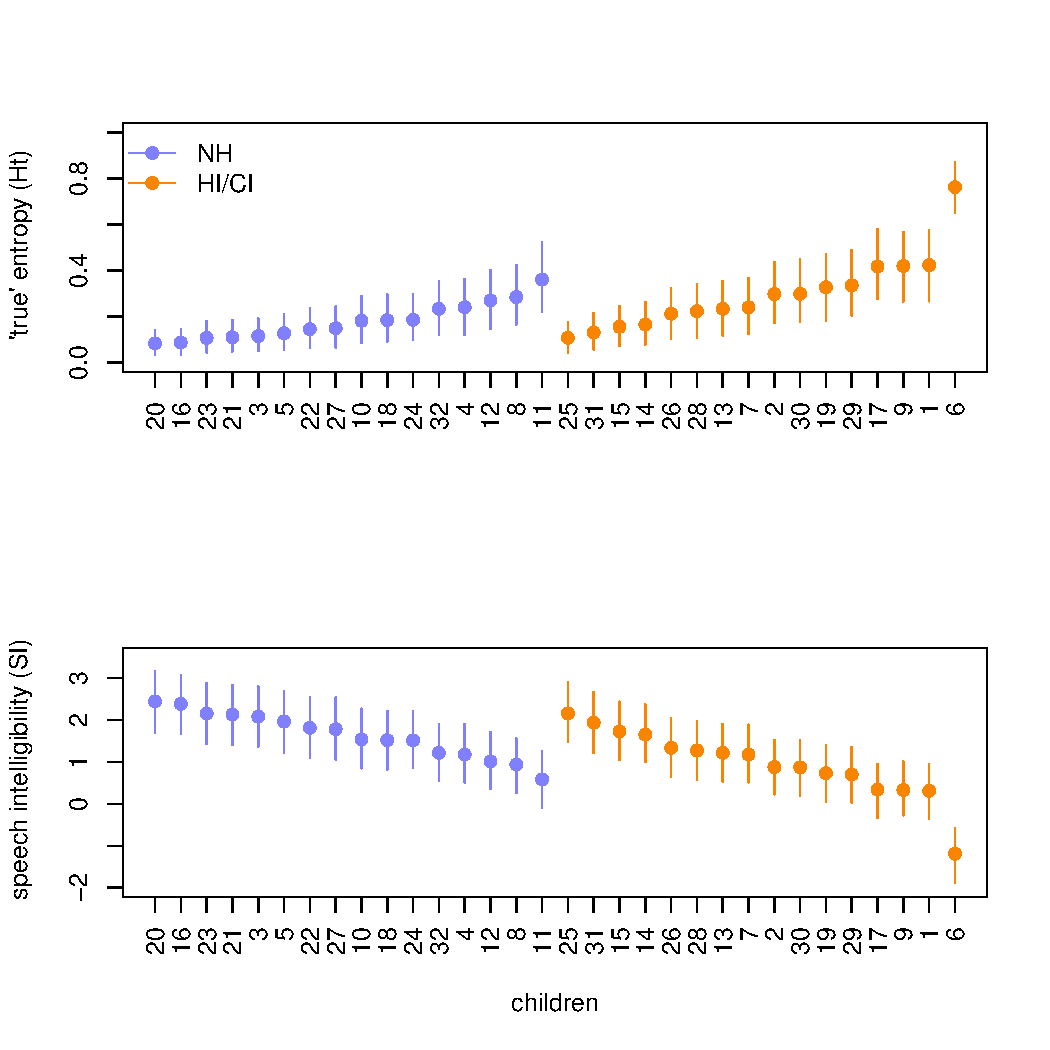
\includegraphics[width=0.7\linewidth]{posterior_predictive_real2.pdf}
	\caption[Posterior predictive: ``true'' entropy and intelligibility scales]{Posterior predictive: ``true'' entropy and speech intelligibility scales}
	\label{fig:predictive2}
\end{figure}
%
\begin{figure}[!h]
	\centering
	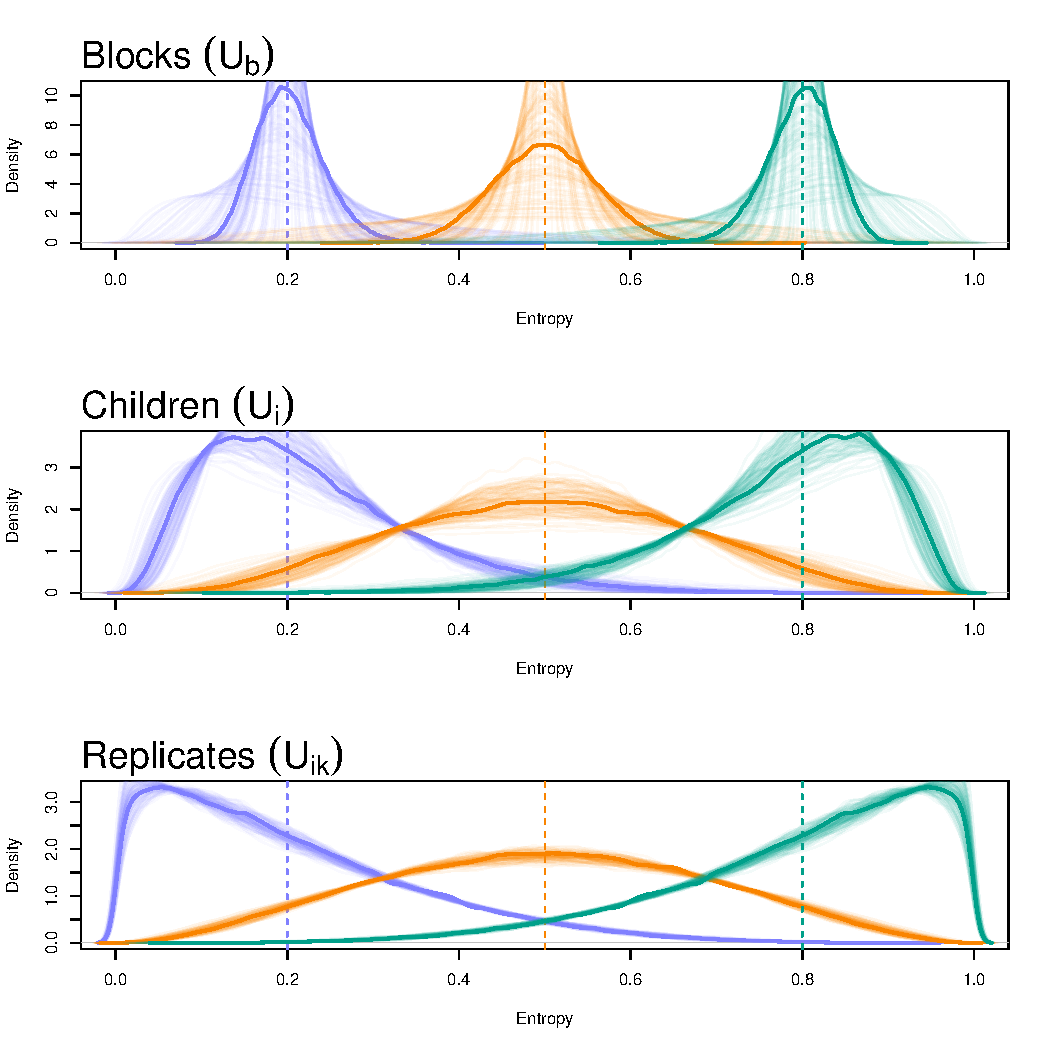
\includegraphics[width=0.5\linewidth]{variability_plot.pdf}
	\caption[Posterior predictive: levels of variability]{Posterior predictive: levels of variability}
	\label{fig:variability}
\end{figure}
%
%
%###############################
\subsection{Posterior predictive} \label{sS:results_posterior}
%###############################
%
\textcolor{red}{work in progress}
%
\begin{figure}[!h]
	\centering
	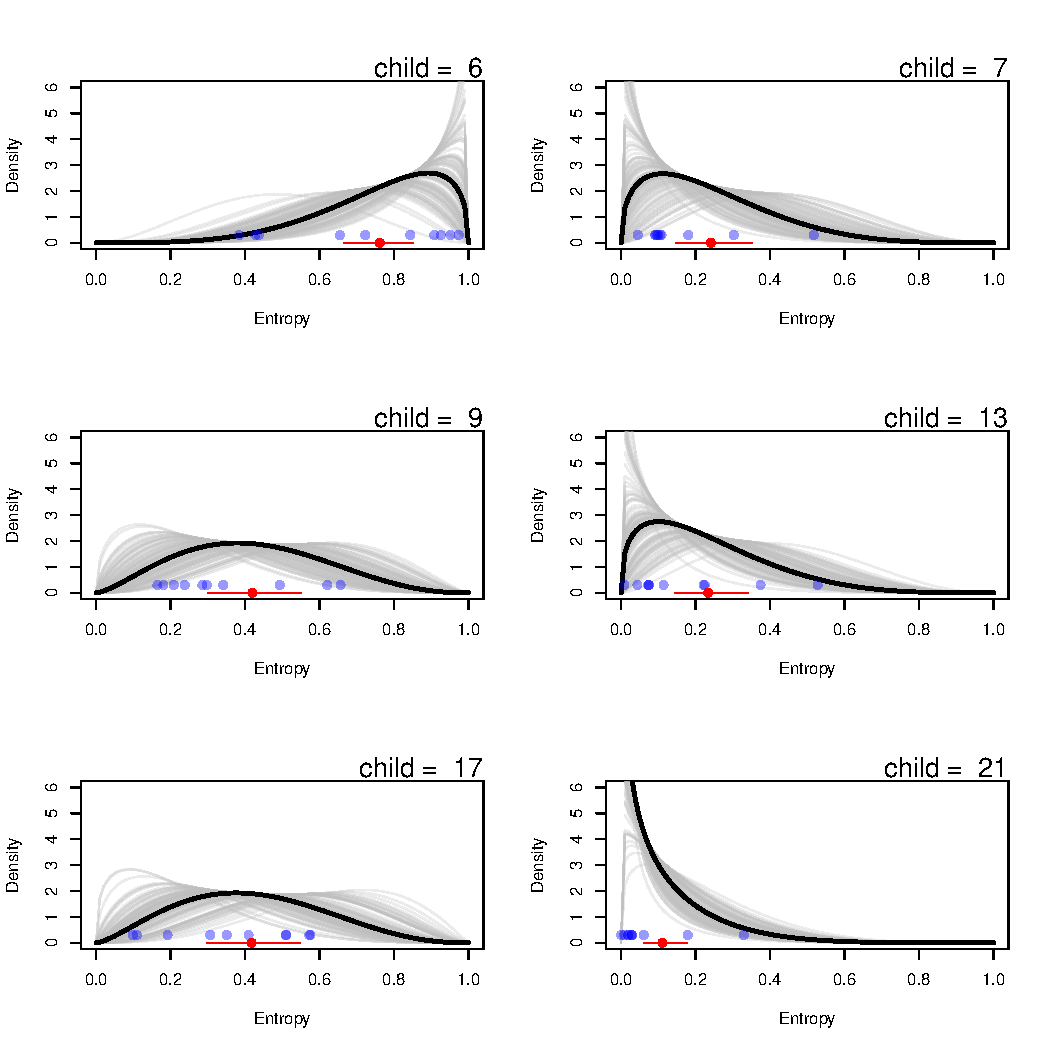
\includegraphics[width=0.7\linewidth]{posterior_predictive_real1.pdf}
	\caption[Posterior predictive: entropy replicates]{Posterior predictive: entropy replicates}
	\label{fig:predictive1}
\end{figure}
%
%
%###############################
\subsection{Outlying observations} \label{sS:results_outliers}
%###############################
%
\textcolor{red}{work in progress}
%
\begin{figure}[!h]
	\centering
	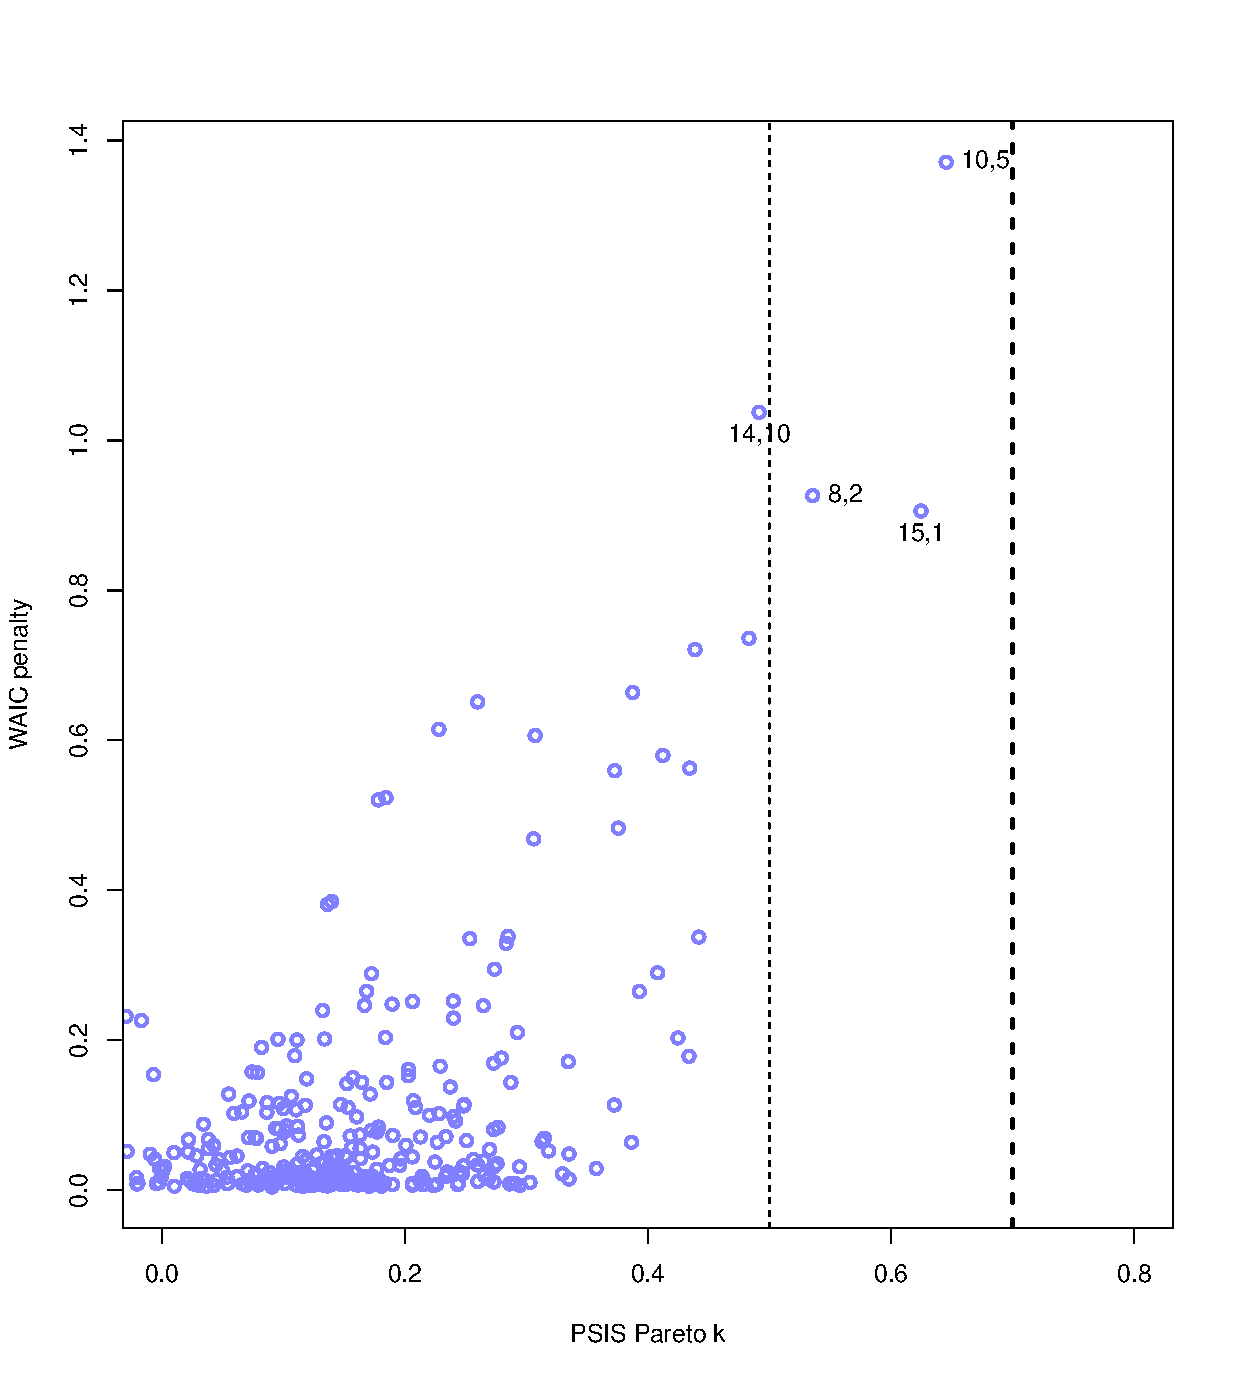
\includegraphics[width=0.5\linewidth]{outliers.pdf}
	\caption[Outlying observations]{Outlying observations. Pairs (child, utterance) are reported for specific observations.}
	\label{fig:outliers}
\end{figure}
%
%